\begin{name}
	{\tenchude}
	{ĐỀ ÔN TẬP CHƯƠNG I}
	{LỚP TOÁN THẦY PHÁT}
	{\thoigian}
\end{name}
\TN
\setcounter{ex}{0}
\Opensolutionfile{ans}[ans021]


%%%% Câu 1
\begin{ex}
	Phát biểu nào sau đây là một mệnh đề toán học?
	\choice
	{Hình vuông đẹp hơn hình tròn}
	{$3$ có phải là số dương không?}
	{$x-2y<3$}
	{\True Số $2024$ là số tự nhiên lẻ}
	\loigiai{
		Phát biểu \lq\lq  Số $2024$ là số tự nhiên lẻ \rq\rq\ là mệnh đề toán học}
\end{ex}

%%%% Câu 2
\begin{ex}
	Câu nào sau đây không là mệnh đề?
	\choice
	{Tam giác đều là tam giác có ba cạnh bằng nhau}
	{$3<1$}
	{$4-5=1$}
	{\True Bạn học giỏi quá!}
	\loigiai{
		Vì “Bạn học giỏi quá!” là câu cảm thán không có khẳng định đúng hoặc sai}
\end{ex}

%%%% Câu 3
\begin{ex}
	Mệnh đề phủ định của mệnh đề “$2024$ là số tự nhiên chẵn” là
	\choice
	{$2024$ là số chẵn}
	{$2024$ là số nguyên tố}
	{\True $2024$ không là số tự nhiên chẵn}
	{$2024$ là số chính phương}
	\loigiai{
		Mệnh đề phủ định của mệnh đề “$2018$ là số tự nhiên chẵn” là “$2018$ không là số tự nhiên chẵn”. }
\end{ex}

%%%% Câu 4
\begin{ex}
	Tìm mệnh đề phủ định của mệnh đề: $\forall x\in \mathbb{R}, \ x^2+x+5>0$.
	\choice
	{$\exists x\in \mathbb{R}, \ x^2+x+5<0$}
	{$\forall x\in \mathbb{R}, \ x^2+x+5<0$}
	{$\forall x\in \mathbb{R}, \ x^2+x+5\leqslant 0$}
	{\True $\exists x\in \mathbb{R}, \ x^2+x+5\leqslant 0$}
	\loigiai{
		$\forall x\in \mathbb{R}, \ x^2+x+5>0$. Suy ra mệnh đề phủ định là $\exists x\in \mathbb{R}, \ x^2+x+5\leqslant 0$}
\end{ex}

%%%% Câu 5
\begin{ex}
	Cho mệnh đề: “ Có một học sinh trong lớp 10A không thích học môn Toán”. Mệnh đề phủ định của mệnh đề này là:
	\choice
	{\True “ Mọi học sinh trong lớp 10A đều thích học môn Toán”}
	{“ Mọi học sinh trong lớp 10A đều không thích học môn Toán”}
	{“ Mọi học sinh trong lớp 10A đều thích học môn Văn”}
	{“ Có một học sinh trong lớp 10A thích học môn Toán”}
	\loigiai{
		Phủ định của mệnh đề: “Có một học sinh trong lớp 10A không thích học môn Toán” là mệnh đề “Mọi học sinh trong lớp 10A đều thích học môn Toán”}
\end{ex}

%%%% Câu 6
\begin{ex}
	Cho $A=\{x\in \mathbb{N}^*\ \mid\ x<10, \ x\vdots 3\}$. Chọn khẳng định đúng.
	\choice
	{$A$ có $4$ phần tử}
	{\True $A$ có $3$ phần tử}
	{$A$ có $5$ phần tử}
	{$A$ có $2$ phần tử}
	\loigiai{
		Ta có $A=\left\{x\in \mathbb{N}^*|x<10, \ x\vdots 3\right\}=\{3;6;9\}$. Suy ra $A$ có $3$ phần tử}
\end{ex}

%%%% Câu 7
\begin{ex}
	Hãy liệt kê các phần tử của tập hợp $X=\left\{x\in \mathbb{R}\ \mid \ 2x^2-5x+3=0\right\}$.
	\choice
	{$X=\{1\}$}
	{$X=\left\{\dfrac{3}{2}\right\}$}
	{$X=\{0\}$}
	{\True $X=\left\{1;\dfrac{3}{2}\right\}$}
	\loigiai{
		Các phần tử của tập hợp $X=\left\{x\in \mathbb{R}\;|\;2x^2-5x+3=0\right\}$ là các nghiệm của phương trình $$2x^2-5x+3=0 \Leftrightarrow \left[\begin{aligned}
			&x=1\\
			&x=\dfrac{3}{2}.\\
		\end{aligned}\right. $$}
\end{ex}

%%%% Câu 8
\begin{ex}
	Cho tập hợp $A=\{a, b, c, d\}$. Tập $A$ có mấy tập con?
	\choice
	{$15$}
	{$12$}
	{\True $16$}
	{$10$}
	\loigiai{
		Số tập hợp con của tập hợp có $4$ phần tử là $2^4=16$ tập hợp con}
\end{ex}

%%%% Câu 9
\begin{ex}
	Cho hai tập hợp $X=\{1;2;4;7;9\}$ và $X=\{-1;0;7;10\}$. Tập hợp $X\cup Y$ có bao nhiêu phần tử?
	\choice
	{$9$}
	{$7$}
	{\True $8$}
	{$10$}
	\loigiai{
		Ta có $X\cup Y=\{-1;0;1;2;4;7;9;10\}$. Do đó $X\cup Y$ có $8$ phần tử}
\end{ex}

%%%% Câu 10
\begin{ex}
	Cho hai tập hợp $A=[-2;3]$ và $B=(1;+\infty)$. Tìm $A\cap B$.
	\choice
	{$A\cap B=[-2;+\infty)$}
	{\True $A\cap B=(1;3]$}
	{$A\cap B=[1;3]$}
	{$A\cap B=(1;3)$}
	\loigiai{
		Biểu diễn hai tập hợp $A$ và $B$ ta được:
		\begin{center}
			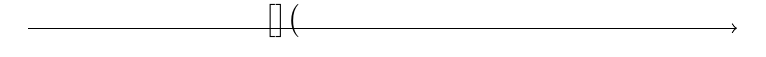
\begin{tikzpicture}
				\draw[->](-3,0)->(6,0);
				%	\IntervalL{}{-3}{[}{-2}
				\IntervalLR{-3}{-2}
				\IntervalGR{}{}{\big[}{-2}
				\IntervalLR{3}{5.9}
				\IntervalGR{\big]}{3}{}{}
				\IntervalLR{-3}{1}
				\IntervalGL{}{}{\big(}{1}
			\end{tikzpicture}
		\end{center}
		Vậy $A\cap B=(1;3]$.
	}
\end{ex}

%%%% Câu 11
\begin{ex}
	Cho $A$, $B$ là hai tập hợp bất kì. Phần tô màu trong hình vẽ bên dưới là tập hợp nào sau đây?\\
	\begin{center}
		% Definition of circles
		\def\firstcircle{(0,0) circle (1.5cm)}
		\def\secondcircle{(0:2cm) circle (1.5cm)}

		\colorlet{circle edge}{blue!50}
		\colorlet{circle area}{blue!20}

		\tikzset{filled/.style={fill=circle area, draw=circle edge, thick},
			outline/.style={draw=circle edge, thick}}

		\setlength{\parskip}{5mm}
		% Set A and B
		\begin{tikzpicture}
			\begin{scope}
				\clip \firstcircle;
				\fill[green!40] \secondcircle;
			\end{scope}
			\draw[outline] \firstcircle node {$A$};
			\draw[outline] \secondcircle node {$B$};
		\end{tikzpicture}
	\end{center}
	\choice
	{$A\cup B$}
	{$B\setminus A$}
	{$A\setminus B$}
	{\True $A\cap B$}
	\loigiai{
		Theo biểu đồ Ven thì phần gạch sọc trong hình vẽ là tập hợp $A\cap B$}
\end{ex}

%%%% Câu 12
\begin{ex}
	Cho các tập hợp $M=[-3;6]$ và $N=(-\infty; -2)\cup (3;+\infty)$. Khi đó $M\cap N$ là
	\choice
	{$(-\infty;-2)\cup (3;6)$}
	{$(-\infty;-2)\cup [3;+\infty)$}
	{\True $[-3;-2)\cup (3;6]$}
	{$(-3;-2)\cup (3;6)$}
	\loigiai{
		Biểu diễn trục số:
		\begin{center}
			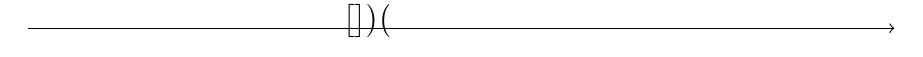
\begin{tikzpicture}
				\draw[->](-4,0)->(7,0);
				\IntervalLR{-4}{-3}
				\IntervalGR{}{}{\big[}{-3}
				\IntervalLR{6}{6.9}
				\IntervalGR{\big]}{6}{}{}
				\IntervalLR{-2}{3}
				\def\skipInterval{0.5cm}
				\IntervalGLF{\big)}{-2}{\big(}{3}
			\end{tikzpicture}
		\end{center}
		Từ hình vẽ, ta có
		Khi đó: $M\cap N= [-3;-2)\cup (3;6]$}
\end{ex}
\Closesolutionfile{ans}
\TNTF
\setcounter{ex}{0}
\Opensolutionfile{ans}[ans022]

%%%% Câu 13
\begin{ex}
	Xét tính đúng sai của các mệnh đề sau
	\choiceTF
	{\True Chu vi của đường tròn có đường kính bằng $10 cm$ là $10\pi$}
	{Hình bình hành có hai cạnh kề bằng nhau là hình vuông}
	{Tam giác có một góc bằng 60 độ là tam giác đều}
	{Diện tích hình vuông có cạnh bằng $3$ là $6$}
	\loigiai
	{
	a)	Ta có đường tròn có đường kính bằng $10 cm$ thì bán kính $r=5 cm$ , do đó có chu vi là $2r\pi=10\pi$ nên mệnh đề đúng.\\
	b)	Hình bình hành có hai cạnh kề bằng nhau là hình thoi, nên mệnh đề sai. \\
	c)	Tam giác cân có một góc bằng $60$ độ là tam giác đều nên mệnh đề sai.\\
	d) Hình vuông có cạnh bằng $3$ thì có diện tích là $9$ nên mệnh đề sai
	}
\end{ex}

%%%% Câu 14
\begin{ex}
	Cho tam giác $ABC$. Xét tính đúng sai của các mệnh đề sau
	\choiceTF
	{\True Tổng của hai cạnh một tam giác lớn hơn cạnh thứ ba}
	{\True Nếu tam giác $ABC$ cân tại $A$ thì $AB=AC$}
	{Nếu một tam giác có một góc bằng 60 độ thì nó là tam giác đều}
	{\True Nếu tam giác $ABC$ vuông tại $C$ thì $AC^2+BC^2=AB^2$}

	\loigiai
	{
	a) Đúng vì tính chất bất đẳng thức về độ dài 3 cạnh của một tam giác.\\
	b)  Đúng vì tính chất của tam giác cân\\
	c) Sai vì tam giác đều có ba góc đều bằng $60^0$.\\
	d) Đúng vì thỏa mãn định lý Pitago
     	}
\end{ex}

%%%% Câu 15
 \begin{ex}
 	Cho hai tập hợp $A=\{a; b\}$ và  $B=\{a;b;c;d\}$. Xét tính đúng sai của các mệnh đề sau
	\choiceTF
 	{\True Tâp hợp $B$ có đúng $4$ phần tử}
 	{Tập hợp $A$ có đúng $4$ tập con khác rỗng}
 	{Số phần tử của tập hợp $A\cap B$ là $4$}
 	{\True Số tập tập $X$ thỏa mãn $A\subset X\subset B$ là $4$}
 	\loigiai
 	{
 	a) Đúng. Tâp hợp $B$ có đúng $4$ phần tử.\\
 	b) Sai. Tập hợp $A$ có đúng $3$ tập con khác rỗng đó là $\{a\}$, $\{b\}$ và $\{a,b\}$.\\
 	c) Sai. Số phần tử của tập hợp $A\cap B=\{a;b\}$ là $2$.\\
 	d) Đúng. Các tập $X$ thỏa mãn $A\subset X\subset B$ là $\{a ; b\}$, $\{a ; b ; c\}$, $\{a ; b ; d\}$, $\{a ; b ; c ; d\}$.
    }
 \end{ex}

 %%%% câu 16
 \begin{ex}
 	Cho hai tập hợp $A=[-2;3]$ và $B=(1;+\infty)$. Xét tính đúng sai các mệnh đề sau.
	\choiceTF
 	{\True Phần tử $1$ thuộc tập hợp $A$}
 	{Phần tử $1$ thuộc tập hợp $B$}
 	{\True Tập hợp $A \cap B = (1; 3]$}
 	{\True Tập hợp $A \cup B = [-2; +\infty)$}
 	\loigiai
 	{
 	a) Đúng. Phần tử $1$ thuộc tập hợp $A$.\\
 	b) Sai. Phần tử $1$ không thuộc tập hợp $B$.\\
 	c) Đúng. Tập hợp $A \cap B = (1; 3]$.\\
 	d) Đúng. Tập hợp $A \cup B = [-2; +\infty)$
 	}
 \end{ex}
\Closesolutionfile{ans}
\TNSA
\setcounter{ex}{0}
\Opensolutionfile{ans}[ans023]

%%%% câu 17
\begin{ex}
	Cho hai tập hợp $X=\{-1;2;4;7;9\}$ và $Y=\{-1;0;7;9;10\}$. Liệt kê các phần tử của tập hợp $X\cap Y$ (thứ tự tăng dần).
	\shortans{-179}
	\loigiai
	{
	Ta có $X\cap Y=\{-1;7;9\}$.
		}
\end{ex}

%%%% Câu 18
\begin{ex}
	Cho tập $A=\{0;2;4;6;8\}$; $B=\{3;4;5;6;7\}$. Số tập hợp con của tập $A\setminus B$ là $m$. Tính $m^4$.
	\shortans{4096}
	\loigiai
	{
	Ta có $A\setminus B=\{0;2;8\}$ nên tập hợp $A\setminus B$ có $2^3=8$ tập hợp con.
	}
\end{ex}

%%%% Câu 19
\begin{ex}
	Cho $A=(-\infty;3m)$, $B=[-5;+\infty)$. Tập tất cả số $m$ để $A \cap B \ne \varnothing$ là $(a;+\infty)$. Số $a$ làm tròn đến hàng phần chục bằng
	\shortans{-1,7}
	\loigiai
	{
	$A \cap B \ne \varnothing \Leftrightarrow 3m> -5 \Leftrightarrow m> -\dfrac53 \approx -1,7$.
	}
\end{ex}

%%%% Câu 20
\begin{ex}
	Cho hai tập hợp $A=\left\{x\in \mathbb{R}\mid -5<x\leqslant 3\right\}$, $B=(-2; 7)$. Số nguyên lớn nhất và số nguyên nhỏ nhất của tập hợp $A\cap B$ lần lượt bằng $m$, $n$. Làm tròn số $\dfrac{n}{m}$ đến hàng phần chục bằng
	\shortans{-0,3}
	\loigiai
	{
	Ta có $A=\left\{x\in \mathbb{R}\mid -5<x\leqslant 3\right\}=(-5; 3]$ $ \Rightarrow (-5; 3]\cap (-2; 7)=(-2; 3]$.\\
	Số nguyên lớn nhất thuộc tập $A\cap B$ là $3$.\\
	Số nguyên nhỏ nhất thuộc tập $A\cap B$ là $-1$.\\
	Vậy $\dfrac{n}{m} = -\dfrac13 \approx -0,3$.
	}
\end{ex}

%%%% Câu 21
\begin{ex}%[Tex hóa BTN1]%[Trần Nhân Kiệt - pb Dương Phước Sang]%[0D1B4-2]
	Cho hai tập hợp $X$, $Y$ thỏa mãn $X\setminus Y=(-7;15)$ và $X\cap Y=(15;2024)$. Tập $X \cap \mathbb{N}$ có bao nhiêu phần tử?
	\shortans{2023}
	\loigiai
	{
	Ta có $X = (X \setminus Y) \cup (X \cap Y) = (-7;15) \cup (15;2024)$.\\
	Suy ra $X \cap \mathbb{N} = \{0;1;\ldots;14;16;17;\ldots;2023 \}$ nên có $2023$ phần tử.
	}
\end{ex}

%%%% Câu 22
\begin{ex}
	Lớp $10A$ có $7$ học sinh giỏi Toán, $5$ học sinh giỏi Lý, $6$ học sinh giỏi Hoá, $3$ học sinh giỏi cả Toán và Lý, $4$ học sinh giỏi cả Toán và Hoá, $2$ học sinh giỏi cả Lý và Hoá, $1$ học sinh giỏi cả ba môn Toán, Lý, Hoá. Số học sinh giỏi ít nhất một môn (Toán hoặc Lý hoặc Hoá) của lớp $10A$ là $i$. Tính $\sqrt{i}$ (làm tròn đến hàng phần trăm).
	\shortans{3,16}
	\loigiai{
		Vẽ biểu đồ Ven biểu diễn cho mỗi liên hệ giữa các tập hợp học sinh giỏi Toán, Lý, Hoá.
		\immini{Và gọi $a,b,c,x,y,z,m$ là số phần tử của mỗi tập hợp thành phần (như trên hình vẽ).\\
			Theo giả thiết $\left\{\begin{aligned}
				&x+m=3\\
				&y+m=2\\
				&z+m=4\\
				&m=1\\
			\end{aligned}\right. \Leftrightarrow \left\{\begin{aligned}
				&x=2\\
				&y=1\\
				&z=3\\
				&m=1.\\
			\end{aligned}\right. $}
		{\def\firstcircle{(0,0) ellipse (3cm and 2cm)}
			\def\secondcircle{(2.5,1) ellipse (3cm and 2cm)}
			\def\thirdcircle{(3.3,-1.2) ellipse (3cm and 2cm)}
			\colorlet{circle edge}{black}
			\colorlet{circle area}{blue!20}
			\tikzset{filled/.style={fill=circle area, draw=circle edge, thick},
				outline/.style={draw=circle edge, thick}}
			\setlength{\parskip}{5mm}
			\begin{tikzpicture}[scale=0.5]
				\begin{scope}
					\clip \firstcircle;
					\clip \secondcircle;
					\fill[filled] \thirdcircle;
				\end{scope}
				\draw[outline] \firstcircle;
				\draw[outline] \secondcircle;
				\draw[outline] \thirdcircle;
				\node[anchor=south west] at (current bounding box.north) {Toán};
				\node[below right] at (current bounding box.east) {Hoá};
				\node[left] at (current bounding box.west) {Lý};
				\node at (3,1.8){$a$};
				\node at (-1.6,0){$b$};
				\node at (4,-1.6){$c$};
				\node at (0.8,1){$x$};
				\node at (0.9,-1.3){$y$};
				\node at (3.7,0.1){$z$};
				\node at (2,-0.2){$m$};
		\end{tikzpicture}}
		\noindent
		Cũng theo giả thiết $\left\{\begin{aligned}
			&a+x+z+m=7\\
			&b+x+y+m=5\\
			&c+y+z+m=6\\
		\end{aligned}\right. \Rightarrow \left\{\begin{aligned}
			&a=1\\
			&b=1\\
			&c=1.\\
		\end{aligned}\right. $\\
		Vậy số học sinh giỏi ít nhất một trong ba môn Toán, Lý, Hoá là $a+b+c+x+y+z+m=10$. Suy ra $\sqrt{i}\approx 3,16$}
\end{ex}
\Closesolutionfile{ans}

